%--- 21 -------------------------------%
\item\vf{Dans une base de données clé-valeur, il est généralement prévu de rechercher toutes les clés dont
les valeurs satisfont une certaine propriété.}
{\faux}
{La clé étant de type \textit{string}, elle est utilisé pour définir des formats/patterns utilisés pour des recherches efficaces.
\paragraph{COMPLETER[...] slide 27}}


%--- 22 -------------------------------%
\item\vf{Il est possible d’imposer des contraintes sur les domaines des valeurs des paires clé-valeur d’une base de données clé-valeur.}
{}
{COMPLETER [...]}


%--- 23 -------------------------------%
\item\vf{Distribuer les données sur un cluster de machines fait partie des éléments mis en place dans le
monde NoSQL.}
{\vrai}
{Le modèle NoSQL se prête bien à la distribution des données (agrégats) sur différentes machines physiques ( = clusters, architecture en noeuds). 

\paragraph{Intérêts du cluster...} 
\begin{itemize}
\item[$\cdot$] gestion de grandes quantités de données, \textit{scale out}: la capicité de stockage peut être facilement augmentée en ajoutant de nouvelles machines et ce "à chaud" 
\item[$\cdot$] meilleur trafic R/W: la répartition de la charge permet de fluidifier le trafic des requêtes
\item[$\cdot$]résister à des ralentissements, pannes réseaux: les machines peuvent être inscrites chez différents Fournisseurs d'Accès Internet (FAI) et le réseau est de ce fait moins sensible à une éventuelle panne chez un FAI ou une saturation
\end{itemize}
 }


%--- 24 -------------------------------%
\item\vf{Il est possible de faire du sharding de données pour une base de données se trouvant sur une
machine unique.}
{\vrai ? (via machine virtuelle) -> mais complètement inutile}
{Le sharding est une technique de distribution des données qui consiste à répartir la charge entre différents serveurs de façon horizontale ( = [...]).
\paragraph{}
En sharding, les données \textbf{ne sont pas répliquées} et chaque serveur est accessible en \textbf{R/W}. Pour optimiser la distribution, on veillera à rassembler sur un même noeud les données qui sont \textit{accédées ensemble} (probabilité d'accès commun et localisation géographique). C'est le client qui a connaissance de la répartition des données et qui est donc responsable d'interroger la bonne machine.
\begin{figure}[!h]
\center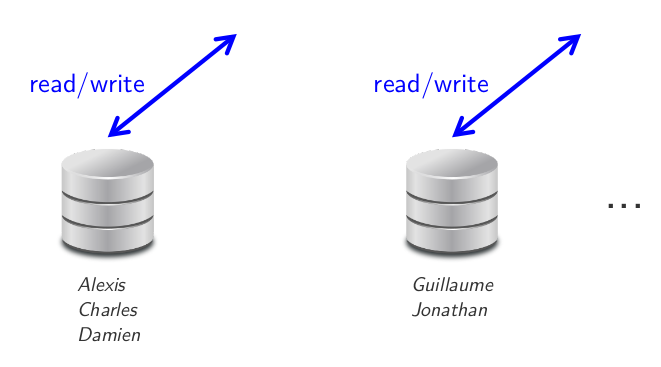
\includegraphics[scale=.3]{images/sharding}
\caption{Distribution des données: modèle sharding \cite{ref1}}
\end{figure}

\paragraph{Avantages:}
\begin{itemize}
\item[$\cdot$]fraction de la DB pour accélérer son traîtement et la rendre plus facile à gérer
\item[$\cdot$]avantages cluster (résistance aux pannes, \textit{scale out}, ...)
\end{itemize}

\paragraph{Inconvénient:}
\begin{itemize}
\item[$\cdot$]définir bonne répartition des données -> risque de surcharge d'un serveur
\item[$\cdot$]pas de résilience (ni en lecture, ni en écriture) -> si un serveur tombe, une partie de la DB n'est plus du tout accessible
\end{itemize}

}


%--- 25 -------------------------------%
\item\vf{Le sharding permet de récupérer les données en cas de corruption grâce à un stockage redondant
de ces dernières sur plusieurs serveurs pouvant être physiquement à des endroits différents.}
{\faux}
{En sharding les données ne sont pas répliquées contrairement aux modèles de réplications \textit{master/slave} ou \textit{peer-to-peer}.}


%--- 26 -------------------------------%
\item\vf{Réplication de données et sharding sont incompatibles.}
{\faux}
{Il est possible de combiner les techniques de \textit{sharding} et \textit{replication} ce qui offre les avantages de résilience (R, W ou les deux) et de répartition de la DB.
\paragraph{}
On peut combiner le sharding avec:
\begin{itemize}
\item[$\cdot$]le \textit{master/slave}: plusieurs maîtres (responsable chacun d'une partie de la DB) ou rôle mixtes (esclave pour certaines données et maîtres pour d'autres)
\item[$\cdot$]le \textit{peer-to-peer}: fraction de la DB (sharding) et réplication sur N noeuds
\end{itemize}
}


%--- 27 -------------------------------%
\item\vf{La réplication master-slave offre la propriété de résilience à la lecture.}
{\vrai}
{Dans le modèle de réplication master/slave, on distingue deux types de noeuds
\begin{enumerate}
\item le \textbf{master}: responsable des données et de leur mise à jour, il est accessible en R/W
\item les \textbf{slaves}: répliques complètes (!!) du maître, accessibles seulement en lecture
\end{enumerate}

\paragraph{}
Les requêtes des clients sont redirigées suivant que ce soit pour de la lecture ou de l'écriture. Comme le master est le seul accessible en lecture, il doit communiquer ses modifications aux esclaves pour les mettre à jour.

\paragraph{}
Ce modèle possède la propriété de \textit{read resilience}, càd que si le maître crash, le système sera toujours accessible en lecture via les esclaves. De plus, il est possible d'élir (manuellement ou automatiquement) un esclave comme nouveau maître si celui-ci tombe.

\begin{figure}[!h]
\center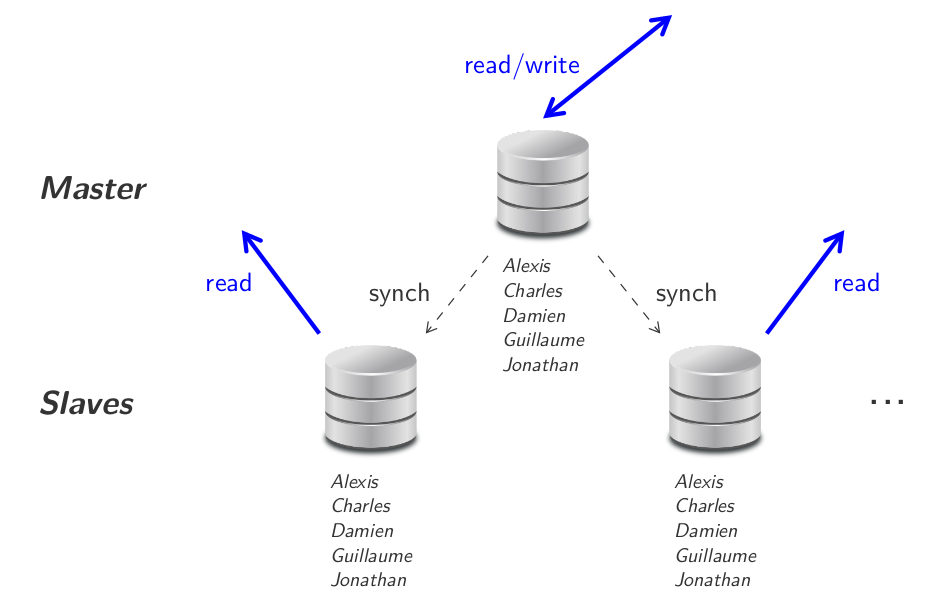
\includegraphics[scale=.3]{images/replication-masterslave}
\caption{Distribution des données: modèle de réplication master/slave \cite{ref1}}
\end{figure}

\paragraph{Avantages:}
\begin{itemize}
\item[$\cdot$]robustesse en cas de crash et \textit{read resilience}
\item[$\cdot$]fluidification du trafic pour les requêtes de lecture
\item[$\cdot$]avantages cluster (résistance aux pannes, \textit{scale out}, ...)
\end{itemize}

\paragraph{Inconvénient:}
\begin{itemize}
\item[$\cdot$]pas adapté lorsqu'il y a beaucoup d'écritures -> surcharge maître
\item[$\cdot$]nécessite plus d'espace de stockage puisque chaque noeud est une copie complète du maître
\item[$\cdot$]les valeurs lues par plusieurs utilisateurs peuvent être différentes par inconsistence -> la cohérence des données n'est pas garantie, puiqu'il faut que le maître ait synchronisé ses modifications avec les esclaves
\end{itemize}
}


%--- 28 -------------------------------%
\item\vf{En utilisant une réplication master-slave, les données deviennent complètement inaccessibles une
fois que le master tombe.}
{\faux}
{Par la propriété de \textit{read resilience}, les données seront toujours accessibles en lecture si le maître crash (avec risque de perte d'information si l'esclave n'était pas à jour par rapport au maître). Elles ne seront disponibles en écriture \textbf{que si} un esclave est désigné pour remplacer le maître (-> pas \textit{write resilience})}


%--- 29 -------------------------------%
\item\vf{La consistence des données est plus compliquées à garantir avec une réplication master-slave
qu’avec une réplication peer-to-peer.}
{\vrai}
{Dans le modèle de réplication \textit{peer-to-peer}, les noeuds sont tous égaux, ils sont \textbf{accessibles en lecture et en écriture}. A chaque écriture sur un noeud, tous les autres doivent être mis à jour, ce qui peut créer des conflits d'écriture concurrente si une même donnée est modifiée à deux endroits différents en même temps.
\begin{figure}[!h]
\center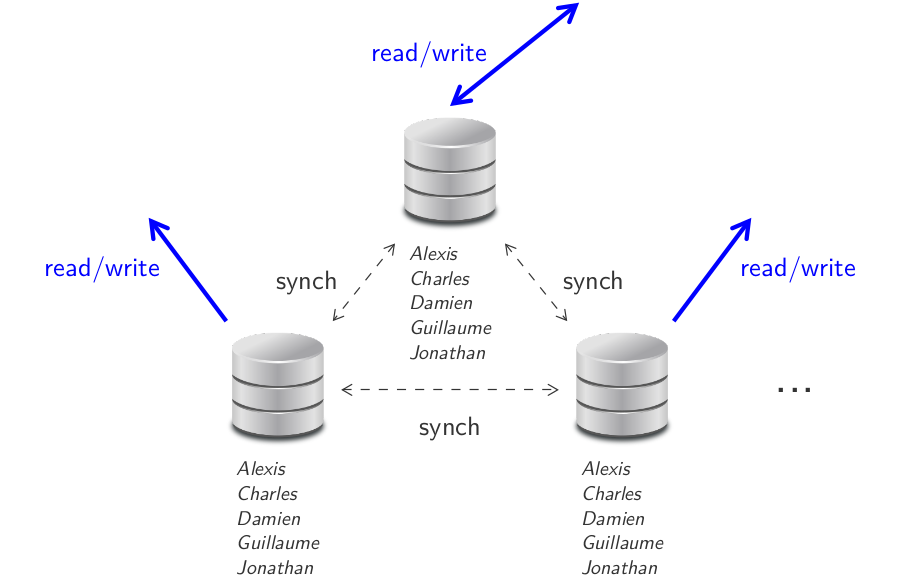
\includegraphics[scale=.3]{images/replication-peertopeer}
\caption{Distribution des données: modèle de réplication peer-to-peer \cite{ref1}}
\end{figure}

\paragraph{Avantages:}
\begin{itemize}
\item[$\cdot$]robustesse en cas de crash et \textit{complete resilience}
\item[$\cdot$]fluidification du trafic pour les requêtes de lecture ET d'écriture
\end{itemize}

\paragraph{Inconvénient:}
\begin{itemize}
\item[$\cdot$]pas adapté lorsqu'il y a beaucoup d'écritures -> lourdeur synchronisations
\item[$\cdot$]nécessite plus d'espace de stockage puisque chaque noeud contient toute la DB
\item[$\cdot$]risques de conflits d'écritures concurrentes
\item[$\cdot$]peu évoluable -> l'ajout d'un nouveau noeud impose de le connecter à TOUS les autres noeuds existants
\end{itemize}
}


%--- 30 -------------------------------%
\item\vf{La consistence des données est plus compliquées à garantir avec une réplication peer-to-peer
qu’avec une réplication master-slave.}
{\faux}
{En master/slave, les modifications peuvent \textbf{seulement} être effectuées via le maître. Il y a donc des risques d'inconsistence des données le temps que les esclaves soient mis à jour MAIS les modifications seront partout les mêmes.
\paragraph{}
En peer-to-peer, des modifications peuvent être faites \textbf{sur n'importe quel noeud} qui communique ensuite à tous les autres ses modifications. Des écritures concurrentes sur différents noeuds peuvent donc engendrer des problèmes d'inconsistence de données qui sont plus difficile à vérifier. (Rem: une solution serait de synchroniser tous les noeuds sur une même date/heure et d'utiliser un serveur dédié pour stocker les informations de mise à jour des données. Ainsi, on peut facilement déterminer la plus récente)
}
